\chapter{Os Limites do Produto}

\section{Limite do Produto}
\hspace{5mm} A forma utilizada para apresentar os limites do produto, consiste num diagrama de use cases, tal como podemos observar nas figuras \ref{img:duc1} \ref{img:duc2}. 

\hspace{5mm}No entanto, importanto referir, que se dividiu o diagrama de use cases em dois subsistemas, para tornar mais fácil a sua avaliação

\begin{figure}[H]
    \centering
	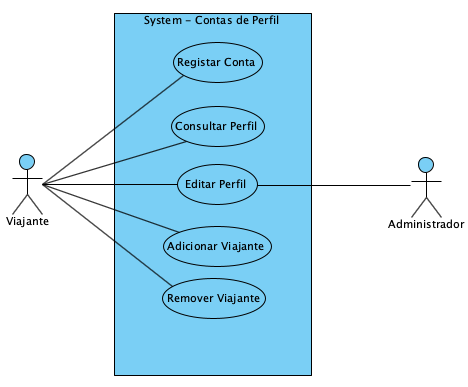
\includegraphics[scale=0.80]{imagens/diagrama-use-cases-1.png}
	\caption{Diagrama de Use cases, do subsistema relacionado com contas de utilizador.}
	\label{img:duc1}
\end{figure}

\begin{figure}[H]
    \centering
	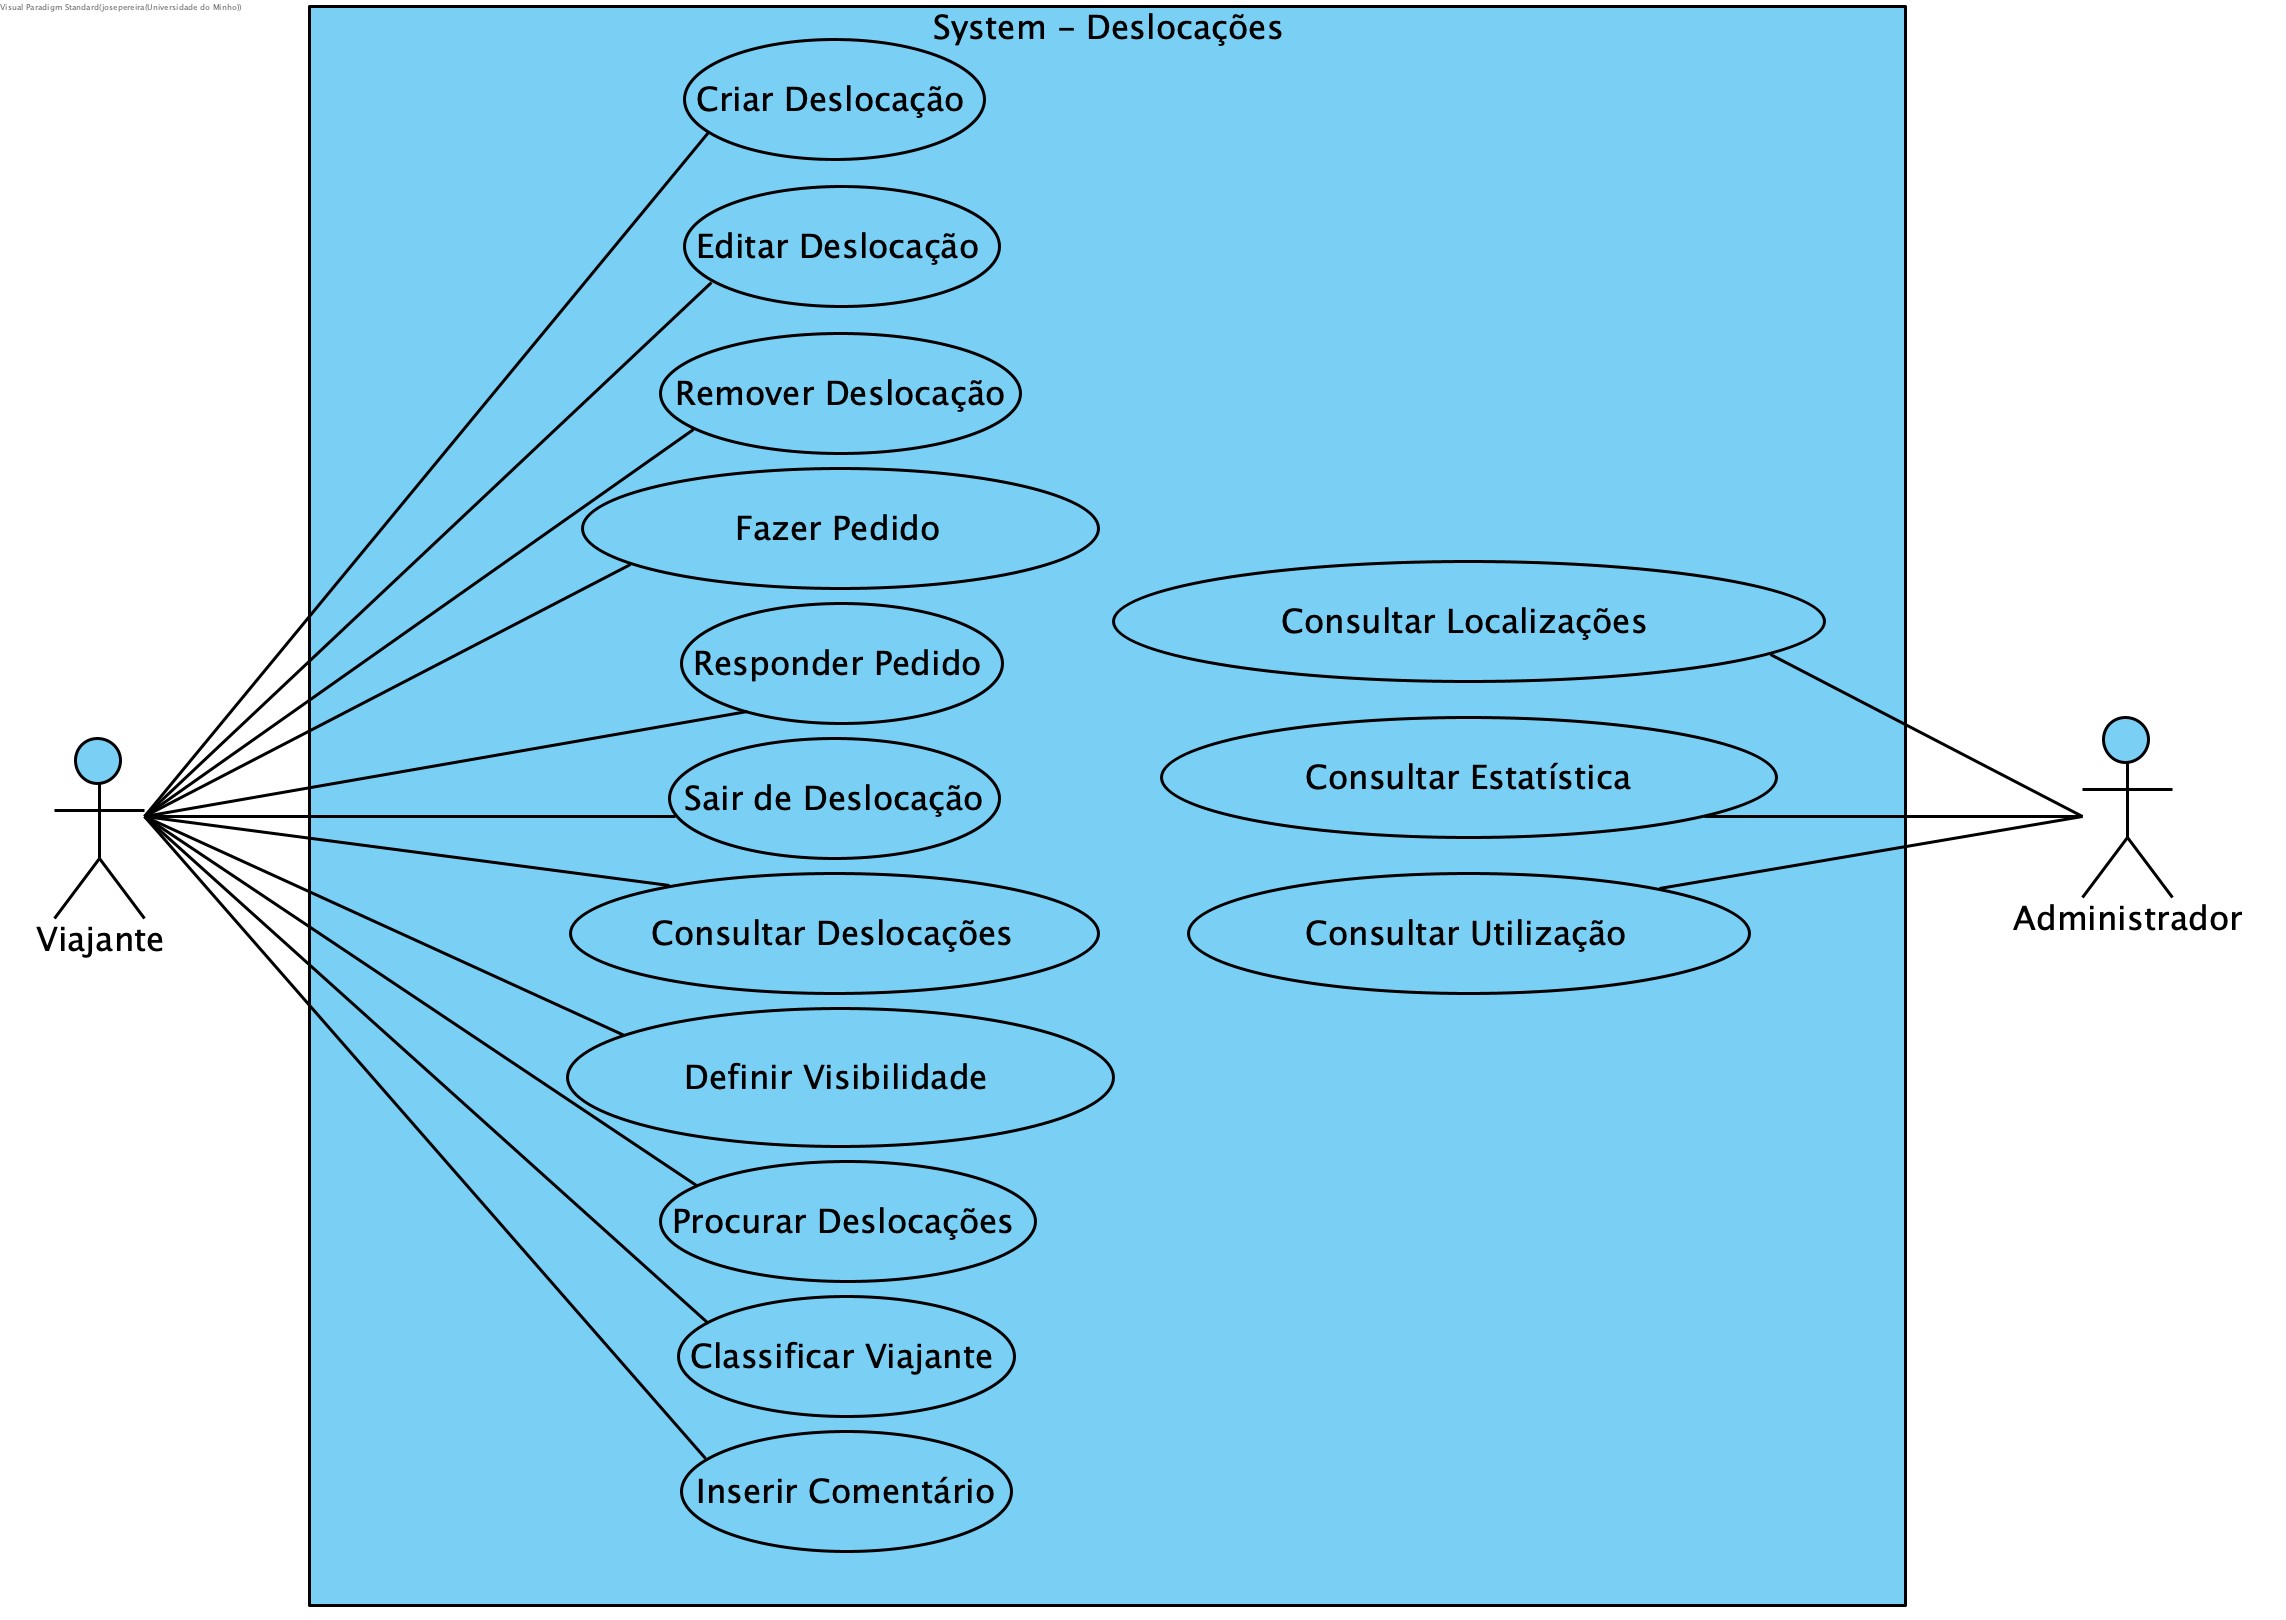
\includegraphics[scale=0.95]{imagens/diagrama-use-cases-2.png}
	\caption{Diagrama de Use cases, do subsistema relacionado com as Deslocações.}
	\label{img:duc2}
\end{figure}

\section{Tabela de \emph{Use Cases} do Produto}
\hspace{5mm} De seguida apresenta-se a tabela, com a identificação dos \emph{use cases}, os atores dos mesmos, bem como os dados de \emph{input} e \emph{output}.

\begin{table}[H]
\begin{center}
\begin{tabularx}{\textwidth}{ | c | c | c | X | }
    \hline
    Número & Nome & Atores & Input/Output \\
    
    \hline
    1 & Registar Conta & Viajante & nome, username, password, email/ mensagem de sucesso ou insucesso \\
    
    \hline
    2 & Consultar Perfil & Viajante & nome ou username/ perfil do viajante dado com input \\
    
    \hline
    3 & Editar Perfil & Viajante e Administrador & campos a serem alterados / sucesso ou insucesso da alteração \\
    
    \hline
    4 & Adicionar Viajante & Viajante & username ou nome do viajante a adicionar à lista de viajantes / sucesso ou insucesso da adição do viajante \\
    
    \hline
    5 & Remover Viajante & Viajante & username ou nome do viajante a remover da lista de viajantes / sucesso ou insucesso da remoção do viajante \\
    
    \hline
    6 & Criar Deslocação & Viajante & data, ponto origem, ponto destino, tipo (frequente, ou não frequente) / sucesso ou insucesso da criação da deslocação \\
    
    \hline
    7 & Editar Deslocação & Viajante & campos a serem alterados (não se pode alterar a origem, destino) / sucesso ou insucesso da edição da deslocação \\
    
    \hline
    8 & Remover Deslocação & Viajante & Identificador (ID) da deslocação / sucesso ou insucesso da remoção da deslocação \\
    
    \hline
    9 & Fazer Pedido & Viajante & ID da deslocação / sucesso ou insucesso da efetuação do pedido \\
    
    \hline
    10 & Responder Pedido & Viajante & aceita ou não aceita / sucesso ou insucesso da efetuação da resposta \\
    
    \hline
    11 & Sair da deslocação & Viajante & Identificador (ID) da deslocação / sucesso ou insucesso da saída da deslocação \\
    
    \hline
    12 & Consultar Deslocações & Viajante & nome ou username do viajante a consultar / lista de deslocações desse viajante \\
    
    \hline
    13 & Definir visibilidade & Viajante & tipo de visibilidade / sucesso ou insucesso da efetuação da operação \\
    
    \hline
    14 & Procurar deslocações & Viajante & filtros (origem, destino, data, tipo, etc...) / lista de deslocações encontradas \\
    
     \hline
    15 & Classificar Viajante & Viajante & valor entre zero e dez / sucesso ou insucesso da efetuação da classificação \\
    
     \hline
    16 & Inserir Comentário & Viajante & comentário / sucesso ou insucesso da inserção do comentário \\
    
     \hline
    17 & Consultar Localizações & Administrador & tipo (mais frequentes ou menos frequentes) / Lista das localizações das deslocações menos ou menos frequentes conforme o input \\
    
     \hline
    18 & Consultar Estatísticas & Administrador & tipo de estatística (métricas a avaliar) / Lista da estatística pedidas como argumento \\
    
    \hline
    19 & Consultar Utilização & Administrador & - / percentagem de utilização inteligente dos veículos total \\
    
    \hline
\end{tabularx}
\end{center}
\label{tab:r1}
\end{table}

\section{\emph{Use Case} Individualmente}

\hspace{5mm} De seguida, apresenta-se, a especificação tabular do \emph{use case} \textbf{Criar Deslocação}. Importa referir, que apenas foi feito a especificação tabular deste \emph{use case}, pois o grupo acha que se trata do mais importante.

\hspace{5mm} Importante referir que no diagrama reutilizou-se a \textbf{Exceção 1} foi usada para os vários casos de valores inválidos, visto que o processo é igual para todos, permitindo assim uma tabela mais pequena.

\newpage

\begin{figure}[H]
    \centering
	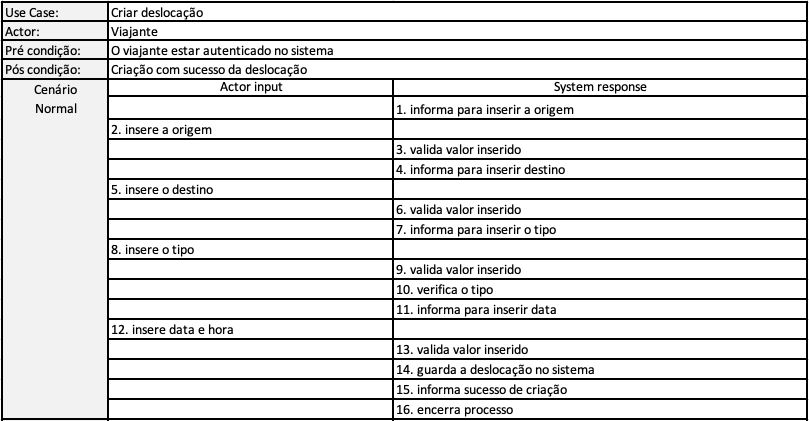
\includegraphics[scale=0.58]{imagens/use-case-especificado-1.png}
	\label{img:duc1}
\end{figure}

\begin{figure}[H]
    \centering
	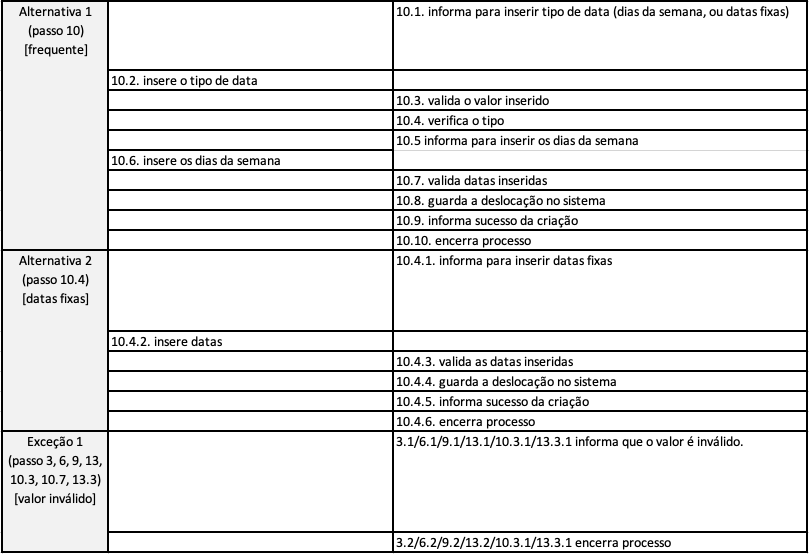
\includegraphics[scale=0.58]{imagens/use-case-especificado-2.png}
	\label{img:duc1}
	\caption{Especificação tabelar do \emph{use case} \textbf{Criar Deslocação}.}
\end{figure}